
%%
%% forked from https://gits-15.sys.kth.se/giampi/kthlatex kthlatex-0.2rc4 on 2020-02-13
%% expanded upon by Gerald Q. Maguire Jr.
%% This template has been adapted by Anders Sjögren to the University
%% Engineering Program in Computer Science at KTH ICT. Adaptation is the
%% translation of English headings into Swedish as the addition of Swedish
%% text. Original body text is deliberately left in English.


%% set the default lanage to english or swedish by passing an option to the documentclass - this handles the inside tile page
\documentclass[english]{kththesis}

% \usepackage[style=numeric,sorting=none,backend=biber]{biblatex}

\setlength {\marginparwidth }{2cm} %leave some extra space for todo notes
\usepackage{todonotes}

\usepackage[perpage,para,symbol]{footmisc} %% use symbols to ``number'' footnotes and reset which symbol is used first on each page

%% Reduce hyphenation as much as possible
\hyphenpenalty=15000 
\tolerance=1000
% include a variety of packages that are useful

%%----------------------------------------------------------------------------
%%   pcap2tex stuff
%%----------------------------------------------------------------------------
%\usepackage[dvipsnames*,svgnames]{xcolor} %% For extended colors
\usepackage{tikz}
\usetikzlibrary{arrows,decorations.pathmorphing,backgrounds,fit,positioning,calc,shapes}
\usepackage{pgfmath}	% --math engine

%% some additional useful packages
\usepackage{rotating}		%% For text rotating
\usepackage{array}		%% For table wrapping
\usepackage{graphicx}	        %% Support for images
\usepackage{float}		%% Suppor for more flexible floating box positioning
\usepackage{mdwlist}            %% various list-related commands
\usepackage{setspace}           %% For fine-grained control over line spacing
\usepackage{listings}		%% For source code listing
\usepackage{bytefield}          %% For packet drawings
\usepackage{tabularx}		%% For simple table stretching
\usepackage{multirow}	        %% Support for multirow colums in tables

\usepackage{url}                %% Support for breaking URLs
\usepackage{hyperref}
\usepackage[all]{hypcap}	%% prevents an issue related to hyperref and caption linking
%% setup hyperref to use the darkblue color on links
\hypersetup{colorlinks,breaklinks,
            linkcolor=darkblue,urlcolor=darkblue,
            anchorcolor=darkblue,citecolor=darkblue}


%% Some definitions of used colors
\definecolor{darkblue}{rgb}{0.0,0.0,0.3} %% define a color called darkblue
\definecolor{darkred}{rgb}{0.4,0.0,0.0}
\definecolor{red}{rgb}{0.7,0.0,0.0}
\definecolor{lightgrey}{rgb}{0.8,0.8,0.8} 
\definecolor{grey}{rgb}{0.6,0.6,0.6}
\definecolor{darkgrey}{rgb}{0.4,0.4,0.4}
\definecolor{aqua}{rgb}{0.0, 1.0, 1.0}

%% If you are going to include source code (or code snippets)
\usepackage{listings}
%%\usepackage[cache=false]{minted} %% For source code highlighting
%%\usemintedstyle{borland}

\usepackage{csquotes} % Recommended by biblatex


%% Acronyms
% note that nonumberlist - removes the cross references to the pages where the acronym appears
% note that nomain - does not produce a main gloassay, this only acronyms will be in the glossary
% note that nopostdot - will present there being a period at the end of each entry
\usepackage[acronym, section=section, nonumberlist, nomain, nopostdot]{glossaries}
%\glsdisablehyper
\makeglossaries
%%% Local Variables:
%%% mode: latex
%%% TeX-master: t
%%% End:
% note the use of a non-breaking dash in long text for the following acronym
\newacronym{IQL}{IQL}{Independent Q‑Learning}

\newacronym{LAN}{LAN}{Local Area Network}
% note the use of a non-breaking dash in the following acronym
\newacronym{WiFi}{Wi-Fi}{Wireless Fidelity}

\newacronym{WLAN}{WLAN}{Wireless Local Area Network}
\newacronym{UN}{UN}{United Nations}
\newacronym{SDG}{SDG}{Sustainable Development Goal}
                %load the acronyms file

%% definition of new command for bytefield package
\newcommand{\colorbitbox}[3]{%
	\rlap{\bitbox{#2}{\color{#1}\rule{\width}{\height}}}%
	\bitbox{#2}{#3}}

\newenvironment{swedishnotes}%
  {\begin{center}
      \selectlanguage{swedish}
      \color{blue}}%
    {\end{center}\selectlanguage{english}
    }

%% Personal commands
% For simpler mathematical expressions and equations.
\newcommand{\X}{\mathcal{X}}
\newcommand{\U}{\mathcal{U}}
\renewcommand{\L}{\mathcal{L}}
\renewcommand{\S}{\mathcal{S}}
\newcommand{\R}{\mathbb{R}}
  
\begin{document}
\selectlanguage{english}


%% Information for inside title page
\title{Predictive Safety Filter for Learning Controllers on Changing Dynamics}
\subtitle{Safety guarantee for reinforcement learning controllers with uncertain dynamics}

% give the alternative title - i.e., if the thesis is in English, then give a Swedish title
\alttitle{Prediktivt säkerhetsfilter för lärande kontroller med förändrande dynamik}
\altsubtitle{Säkerhetsgaranti för förstärkningsinlärning kontroller med okänd dynamik}

\authorsLastname{Liu}
\authorsFirstname{John}
\email{johnliu@kth.se}
\kthid{u100001}
% If the student has an ORCiD - add it here
% \orcid{0000-0002-00001-1234}
\authorsSchool{\schoolAcronym{EECS}}

\supervisorAsLastname{Proutiere}
\supervisorAsFirstname{Alexandre}
\supervisorAsEmail{alepro@kth.se}
% If the supervisor is from within KTH add their KTHID, School and Department info
\supervisorAsKTHID{u100003}
\supervisorAsSchool{\schoolAcronym{EECS}}
\supervisorAsDepartment{Computer Science}
% other for a supervisor outside of KTH add their organization info
%\supervisorAsOrganization{Timbuktu University, Department of Pseudoscience}

%If there is a second supervisor add them here:
% \supervisorBsLastname{Proutiere}
% \supervisorBsFirstname{Alexandre}
% \supervisorBsEmail{sb@kth.se}
% If the supervisor is from within KTH add their KTHID, School and Department info
% \supervisorBsKTHID{u100003}
% \supervisorBsSchool{\schoolAcronym{ABE}}
% \supervisorBsDepartment{Public Buildings}
% other for a supervisor outside of KTH add their organization info
%\supervisorBsOrganization{Timbuktu University, Department of Pseudoscience}

\examinersLastname{Rojas}
\examinersFirstname{Cristian}
\examinersEmail{crro@kth.se}
% If the examiner is from within KTH add their KTHID, School and Department info
\examinersKTHID{u100004}
\examinersSchool{\schoolAcronym{EECS}}
\examinersDepartment{Computer Science}
% other for a examiner outside of KTH add their organization info
%\examinersOrganization{Timbuktu University, Department of Pseudoscience}


\hostcompany{Einride AB} % Remove this line if the project was not done at a host company
%\hostorganization{CERN}   % if there was a host organization

\date{\today}

\programcode{TSCRM}
%% Alternatively, you can say \programme{Civilingenjör Datateknik} to directly set the programme string

\titlepage
% document/book information page
\bookinfopage

% Frontmatter includes the abstracts and table-of-contents
\frontmatter
\setcounter{page}{1}
\begin{abstract}
  \markboth{\abstractname}{}
  \todo[inline]{The first abstract should be in the language of the thesis.}

\todo[inline]{Keep in mind that most of your potential readers are only going to read your title and abstract. This is why it is important that the abstract give them enough information that they can decide is this document relevant to them or not. Otherwise the likely default choice is to ignore the rest of your document.\\
A abstract should stand on its own, i.e., no citations, cross references to the body of the document, acronyms must be spelled out, …\\
Write this early and revise as necessary. This will help keep you focused on what you are trying to do.}

Write an abstract\todo{Use about 1/2 A4-page (250 and 350 words).}  with the following components:
\begin{itemize}
  \item What is the topic area? (optional) Introduces the subject area for the project.
  \item Short problem statement
  \item Why was this problem worth a Master’s thesis project? (i.e., why is the problem both significant and of a suitable degree of difficulty for a Master’s thesis project? Why has no one else solved it yet?)
  \item How did you solve the problem? What was your method/insight?
  \item Results/Conclusions/Consequences/Impact: What are your key results/conclusions? What will others do based upon your results? What can be done now that you have finished - that could not be done before your thesis project was completed?\todo[inline]{The presentation of the results should be the main part of the abstract.}
\end{itemize}

\subsection*{Keywords}
Safe learning, Reinforcement learning, Model predictive control

Choose the most specific keyword from those used in your domain, see for example:
ACM's Computing Classification System (2012) or
(2014) IEEE Taxonomy. 

Mechanics:
\begin{itemize}
  \item The first letter of a keyword should be set with a capital letter and proper names should be capitalized as usual.
  \item Spell out acronyms and abbreviations.
  \item Avoid "stop words" - as they generally carry little or no information.
  \item List your keywords separated by commas (",").
\end{itemize}    
Since you should have both English and Swedish keywords - you might think of ordering them in corresponding order (i.e., so that the nth word in each list correspond) - thus it would be easier to mechanically find matching keywords.


\end{abstract}
\cleardoublepage

\selectlanguage{swedish}
  \begin{abstract}
    \markboth{\abstractname}{}
    \todo[inline]{All theses at KTH are required to have an abstract in both English and Swedish.\\
If you are writing your thesis in English, you can leave this until the final version. If you are writing your thesis in Swedish then this should be done first – and you should revise as necessary along the way.\\
If you are writing your thesis in English, then this section can be a summary targeted at a more general reader. However, if you are writing your thesis in Swedish, then the reverse is true – your abstract should be for your target audience, while an English summary can be written targeted at a more general audience.\\
This means that the English abstract and Swedish sammnfattning  
or Swedish abstract and English summary need not be literal translations of each other.\\

The abstract in the language used for the thesis should be the first abstract, while the Summary/Sammanfattning in the other language can follow.\\

Exchange students many want to include one or more abstracts in the language(s) used in their home institutions to avoid the neeed to write another thesis when returing to their home institution.
}

\subsection*{Nyckelord}
5-6 nyckelord\todo{Nyckelord som beskriver innehållet i uppsatsrapporten}


  \end{abstract}

\cleardoublepage
\selectlanguage{english}
\section*{Acknowledgments }
\markboth{Acknowledgments}{}
\todo[inline]{It is nice to acknowledge the people that have helped you. It is
  also necessary to acknowledge any special permissions that you have gotten –
  for example getting permission from the copyright owner to reproduce a
  figure. In this case you should acknowledge them and this permission here
  and in the figure’s caption. \\
  Note: If you do not have the copyright owner’s permission, then you cannot use any copyrighted figures/tables/… .
}
\todo[inline, backgroundcolor=aqua]{I detta kapitel kan du e v nämna något om
  din bakgrund om det påverkar rapporten på något sätt. Har du t ex inte
  möjlighet att skriva perfekt svenska för att du är nyanländ till landet kan
  det vara på sin plats att nämna detta här. OBS, detta får dock inte vara en
  ursäkt för att lämna in en rapport med undermåligt språk, grammatik och
  stavning (t ex får fel som en automatisk stavningskontroll och
  grammatikkontroll kan upptäcka inte förekomma)\\

En dualism som måste hanteras i hela rapporten och projektet
}

I would like to thank xxxx for having yyyy.\\

\acknowlegmentssignature

\fancypagestyle{plain}{}
\renewcommand{\chaptermark}[1]{ \markboth{#1}{}} 
\tableofcontents
  \markboth{\contentsname}{}

\cleardoublepage
\listoffigures

\cleardoublepage

\listoftables
\cleardoublepage
\lstlistoflistings
\cleardoublepage
\printglossary[type=\acronymtype, title={List of acronyms and abbreviations}]
\todo[inline]{The list of acronyms and abbreviations should be in alphabetical order based on the spelling of the acronym or abbreviation.
}
\label{pg:lastPageofPreface}
% Mainmatter is where the actual contents of the thesis goes
\mainmatter

\renewcommand{\chaptermark}[1]{\markboth{#1}{}}
\chapter{Introduction}

\begin{itemize}
    \item The world is becoming more autonomized. \textbf{refs}
    \item Transportation of people and goods is a large part of our
        infrastructure. \textbf{refs}
    \item Autonomous driving can reduce costs, improve efficiency and increase
        safety. \textbf{refs}
    \item Traditionally, vehicle motion has been tackled using model-based
        method combined with conventional control theory. \textbf{refs}
    \item The main issue with using model-based solutions is that they cannot
          deal with changing environments (such as different terrain and
          weather conditions). \textbf{refs}
    \item Artificial intelligence has become more prominent during the
          last decades solving advance problems such as \textbf{list and reference
          articles}.
      \item Recently, several machine learning solutions to motion planning
          problems has arrived. \textbf{refs}
    \item However, there machine learning lacks safety guarantees which is
        crucial for a safety critical system. \textbf{refs}
    \item Therefore, a pure machine learning solution is not a viable solution
        for autonomous driving in practice. \textbf{refs}
    \item In this report, we will investigate the viability of using a predictive
        safety filter to ensure safe training of a machine learning motion
        planning controller. \textbf{refs}
    \item Specifically, we are evaluate the predictive safety filer on a path following problems.
\end{itemize}

\todo[inline, backgroundcolor=aqua]{svensk: Introduktion}
\label{ch:introduction}

\todo[inline, backgroundcolor=aqua]{Ofta kommer problemet och problemägaren
  från industrin där man önskar en specifik lösning på ett specifikt
  problem. Detta är ofta ”för smalt” definierat och ger ofta en ”för smal”
  lösning för att resultatet skall vara intressant ur ett mer allmänt
  ingenjörsperspektiv och med ”nya” erfarenheter som resultat. Fundera
  tillsammans med projektets intressenter (student, problemägare och akademi)
  hur man skulle kunna använda det aktuella problemet/förslaget för att
  undersöka någon ingenjörsaspekt och vars resultat kan ge ny eller
  kompletterande erfarenhet till ingenjörssamfundet och vetenskapen.\\
  
  Examensarbetet handlar då om att ta fram denna nya ”erfarenhet” och på köpet
  löser man en del eller hela delen av det ursprungliga problemet.\\

  Erfarenheten kommer ur en frågeställning som man i examensarbetet försöker
  besvara med tidigare och andras erfarenhet, egna eller modifierade metoder som
  ger ett resultat vilket kan användas för att diskutera ett svar på
  undersökningsfrågan.\\

  Detta stycke skall alltså, förutom det ursprungliga ”smala” problemet,
  innehålla  vad som skall undersökas för att skapa ny ingenjörserfarenhet
  och/eller vetenskap.
}

This\todo{The first paragraph after a heading is not indented, all of the
  subsequent paragraphs have their first line indented.} chapter describes the
specific problem that this thesis addresses, the context of the problem, the
goals of this thesis project, and outlines the structure of the thesis.\\

\todo[inline]{Give a general introduction to the area. (Remember to use appropriate references in this and all other sections.)}


%We use the \emph{biblatex} package to handle our references.  We therefore
%use the command \texttt{parencite} to get a reference in parenthesis, like
%this \parencite{heisenberg2015}.  It is also possible to include the author as part of the sentence using \texttt{textcite}, like talking about
%the work of \textcite{einstein2016}.

We use the \emph{bibtex} package to handle our references.  We therefore
use the command \cite{farshin_make_2019}. For example, Farshin, et al. described how to improve LLC
cache performance in \cite{farshin_make_2019} in the context of links running
at \SI{200}{Gbps}.

In this thesis we will examine the use of \glspl{LAN}. In this thesis we will
assume that \glspl{LAN} to include \glspl{WLAN}, such as \gls{WiFi}.

Present the background for the area. Set the context for your project – so that your reader can understand both your project and this thesis. (Give detailed background information in Chapter 2 - together with related work.)
Sometimes it is useful to insert a system diagram here so that the reader
knows what are the different elements and their relationship to each
other. This also introduces the names/terms/… that you are going to use
throughout your thesis (be consistent). This figure will also help you later
delimit what you are going to do and what others have done or will do.

As one can find in RFC 1235\cite{ioannidis_coherent_1991} multicast is useful for xxxx .

\section{Problem}
\todo[inline, backgroundcolor=aqua]{svensk: Problemdefinition elle Frågeställning\\
Lyft fram det ursprungliga problemet om det finns något och definiera därefter
den ingenjörsmässiga erfarenheten eller/och vetenskapen som kan komma ur
projektet. }

Longer problem statement\\
If possible, end this section with a question as a problem statement.

% Research Question
\subsection{Original problem and definition}
\todo[inline, backgroundcolor=aqua]{Ursprungligt problem och definition}

\begin{itemize}
    \item The simulation system is a vehicle.
    \item Take a path described by the curvature function $\gamma(s): [0,
        \infty) \rightarrow \Gamma$, where $s$ is the distance along the path.
    \item We have a reinforcement learning controller that is able to follow
        the path $\gamma(s)$ up to a certain margin of error.
    \item Now, impose additional state constraints that require the vehicle to be
        contained a set distance from the path at all times when training the
        controller.
    \item The reinforcement controller is unable to satisfy the additional
        constraints.
    \item Nevertheless, can we couple a predictive safety filter to system such
        that the constraints are indeed satisfied? And to what extent can a
        predictive safety filter improve the safety during training.
\end{itemize}


\subsection{Scientific and engineering issues}\todo[inline, backgroundcolor=aqua]{Vetenskaplig och ingenjörsmässig frågeställning}
some text

\section{Purpose}
\todo[inline, backgroundcolor=aqua]{Syfte}
State the purpose  of your thesis and the purpose of your degree project.

Describe who benefits and how they benefit if you achieve your goals. Include anticipated ethical, sustainability, social issues, etc. related to your project. (Return to these in your reflections in Section~\ref{sec:reflections}.)

\todo[inline, backgroundcolor=aqua]{Skilj på syfte och mål! Syfte är att förändra något till det bättre. I examensarbetet finns ofta två aspekter på detta. Dels vill problemägaren (företaget) få sitt problem löst till det bättre men akademin och ingenjörssamfundet vill också få nya erfarenheter och vetskap. Beskriv ett syfte som tillfredställer båda dessa aspekter.\\
Det finns även ett syfte till som kan vara värt att beakta och det är att du som student skall ta examen och att du måste bevisa, i ditt examensarbete, att du uppfyller examensmålen. Dessa mål sammanfaller med kursmålen för examensarbetskursen. 
}

\section{Goals}
\todo[inline, backgroundcolor=aqua]{Mål}
\todo[inline, backgroundcolor=aqua]{Skilj på syfte och mål. Syftet är att åstakomma en förändring i något. Målen är vad som konkret skall göras för att om möjligt uppnå den önskade förändringen (syfte). }



State the goal/goals of this degree project.

The goal of this project is XXX. This has been divided into the following three sub-goals:
\begin{enumerate}
\item Subgoal 1 \todo[inline, backgroundcolor=aqua]{för att tillfredsställa problemägaren – industrin?}
\item Subgoal 2\todo[inline, backgroundcolor=aqua]{för att tillfredsställa ingenjörssamfundet och vetenskapen – akademin) }
\item Subgoal 3\todo[inline, backgroundcolor=aqua]{eventuellt, för att uppfylla kursmålen – du som student}
\end{enumerate}

In addition to presenting the goal(s), you might also state what the deliverables and results of the project are. 

\section{Research Methodology}\todo[inline, backgroundcolor=aqua]{Undersökningsmetod}
\todo[inline, backgroundcolor=aqua]{Här anger du vilken vilken övergripande undersökningsstrategi eller metod du skall använda för att försöka besvara den akademiska frågeställning och samtidigt lösa det e v ursprungliga problemet. Ofta kan man använda ”lösandet av ursprungsproblemet” som en fallstudie kring en akademisk frågeställning. Du undersöker någon intressant fråga i ”skarpt” läge och samlar resultat och erfarenhet ur detta.\\
Tänk på att företaget ibland måste stå tillbaka i sin önskan och förväntan på projektets resultat till förmån för ny eller kompletterande ingenjörserfarenhet och vetenskap (ditt examensarbete). Det är du som student som bestämmer och löser fördelningen mellan dessa två intressen men se till att alla är informerade. }
Introduce your choice of methodology/methodologies and method/methods – and the reason why you chose them. Contrast them with and explain why you did not choose other methodologies or methods. (The details of the actual methodology and method you have chosen will be given in Chapter~\ref{ch:methods}. Note that in Chapter~\ref{ch:methods}, the focus could be research strategies, data collection, data analysis, and quality assurance.)\\
In this section you should present your philosophical assumption(s), research method(s), and research approach(es).

\section{Delimitations}\todo[inline, backgroundcolor=aqua]{Avgränsningar}
Describe the boundary/limits of your thesis project and what you are explicitly not going to do. This will help you bound your efforts – as you have clearly defined what is out of the scope of this thesis project. Explain the delimitations. These are all the things that could affect the study if they were examined and included in the degree project.

\section{Structure of the thesis}\todo[inline, backgroundcolor=aqua]{ Rapportens disposition}
Chapter~\ref{ch:background} presents relevant background information about xxx.  Chapter~\ref{ch:methods} presents the methodology and method used to solve the problem. …

\cleardoublepage
\chapter{Background}
\todo[inline, backgroundcolor=aqua]{Bakgrund}
\label{ch:background}
\todo[inline]{When you do your literature study, you should have a nearly complete Chapters 1 and 2.\\
You may also find it convenient to introduce the future work section into your report early – so that you can put things that you think about but decide not to do now into this section.\\
Note that later you can move things between this future work section and what you have done as you may change your mind about what to do now versus what to put off to future work.
}

This chapter provides basic background information about xxx. Additionally, this chapter describes xxx. The chapter also describes related work xxxx.

What does a reader (another x student -- where x is your study line) need to know to understand your report?
What have others already done? (This is the “related work”.) Explain what and
how prior work / prior research will be applied on or used in the degree
project /work (described in this thesis). Explain why and what is not used in
the degree project and give valid reasons for rejecting the work/research.

\todo[inline, backgroundcolor=aqua]{Vilken viktig litteratur och
  (forsknings-)artiklar har du studerat inom området (litteraturstudie)? }

\section{Path Following}

\subsection{Discrete Paths}

\subsection{Frenet-Serret Frame}

\section{Model Predictive Control}

\begin{equation}\begin{split}
    \min_{u \in \U} \quad &x_{N|k}^T Q_N x_{N|k} + \sum_{i=0}^{N-1} x_{i|k}^T Q x_{i|k} + u_{i|k}^T R u_{i|k} \\
    \text{s.t.} \quad &x_{i+1|k} = f(x_{i|k}, u_{i|k}), \quad \text{for} \quad i = 0, 1, \dots, N-1 \\
    &(x_{i|k}, u_{i|k}) \in \X \times \U, \quad \text{for} \quad i = 0, 1, \dots, N-1 \\
    &x_{N|k} \in \X_N
\end{split}\end{equation}

\begin{itemize}
    \item Very effective since it is using an optimal control based approach with a receding horizon.
    \item Downside is that it is based on a predetermined model of system dynamics. Performance is then dependent on the accuracy of the model.
    \item On the other side, using a model-based controller, we can consider input and state constraints while computing the input signals.
    \item Also, since MPC is utilizing a receding horizon the controller has to solve an optimization problem each time step which is very computationally expensive.
\end{itemize}

\section{Reinforcement Learning}

\begin{itemize}
    \item \cite{arulkumaran2017}
    \item Vanilla reinforcement learning do not consider a physical model of the system. Instead, it utilizes a neural network model to perform classification and regression.
    \item The advantage of this approach is that the neural network can, in theory, learn extremely complex and nonlinear systems, while conventional parametric method can only learn linear approximations.
    \item Reinforcement learning is often used for online learning, meaning that the controller do not need to collect preliminary data for offline training.
    \item While this seems very promising one of the biggest challenges with reinforcement learning is that ensure convergence to a global optima, or at least a local optima with a cost close to the global cost.
    \item Another issue with reinforcement learning is that a neural network introduces a multitude of hyperparameters which need to be carefully tuned for good performance. This task can sometimes be seen as more an art form rather than a scientific method.
\end{itemize}

\subsection{Policy Gradient}

\begin{itemize}
    \item \cite{li2019}
    \item Policy gradient is a reinforcement learning method that is applied to systems with discrete actions domains and continuous state domains.
    \item Policy gradient can be used when we want to avoid assuming model dynamics. It instead computes the gradient with respect to network parameters based on the cost on certain actions.
\end{itemize}

\section{Bayesian Linear Regression}

\begin{itemize}
    \item Bayesian linear regression uses prior and likelihood assumptions to estimate posterior and predictive values. This can be used to estimate linear approximations for nonlinear systems.
    \item This method not only estimate the considered system, it also provides an uncertainty  corresponding to each value estimation.
    \item While other linear regression methods can compute the covariance for point in the training data it cannot, however, provide a covariance for unexplored points. Nevertheless, this is possible using bayesian system identification methods.
    \item Additionally, using a bayesian methods, we can model measurement noise in the prior estimation.
\end{itemize}

\section{Predictive Safety Filter}

\begin{equation}\begin{split}
    \min_{u \in \U} \quad &(u_\L - u_{0|k})^2 \\
    \text{s.t.} \quad &x_{i+1|k} = f(x_{i|k}, u_{i|k}), \quad \text{for} \quad i = 0, 1, \dots, N-1 \\
    &(x_{i|k}, u_{i|k}) \in \X \times \U, \quad \text{for} \quad i = 0, 1, \dots, N-1 \\
    &x_{N|k} \in \X_N
\end{split}\end{equation}

\begin{itemize}
    \item \cite{wabersich2021safe}
    \item A predictive safety filter is used as a safeguard for learning controllers, such a reinforcement learning controller based on policy gradient. It applies the same theory as model predictive control to determine if the input signal from the learning controller is safe or not.
    \item If the input signal is unsafe, the safety filter will make necessary adjustments while being as noninvasive as possible to the learning input signal.
    \item With this, the predictive safety filter adopts all benefits from model predictive control and reinforcement learning as well as avoiding several of the disadvantages.
    \item It also decouples performance and safety since the learning controller is responsible for performance and the safety filter is responsible for safety.
\end{itemize}


\section{Major background area 1}\todo[inline, backgroundcolor=aqua]{Viktigt bakgrundsområde 1}
There are xxx characteristics that distinguish yyy from other information and communication technology (ICT) system, as shown in Figure~\ref{fig:lotsofstars}. Table \ref{tab:tablecaracteristics} summarizes these characteristics.

 
\begin{figure}[!ht]
  \begin{center}
    
\includegraphics[width=0.5\textwidth]{lots_of_stars.png}
  \end{center}
  \caption{Lots of stars  (Inspired by Figure x.y on page z of [xxx])}
  \label{fig:lotsofstars}
\end{figure}
\todo[inline, backgroundcolor=aqua]{Massor av stärnor (Inspirerad av figur x.y på sidan z i [xxx])}


\begin{table}[!ht]
  \begin{center}
    \caption{xxx characteristics}
    \label{tab:tablecaracteristics}
    \begin{tabular}{l|S[table-format=4.6]} % <-- Alignments: 1st column left, 2nd middle, with vertical lines in between
      \textbf{Characteristics} & \textbf{Description}\\
      $\alpha$ & $\beta$ \\
      \hline
      1 & 1110.1\\
      2 & 10.1\\
      3 & 23.113231\\
    \end{tabular}
  \end{center}
\end{table}
\todo[inline, backgroundcolor=aqua]{Egenskaper}
\todo[inline, backgroundcolor=aqua]{ Beskrivning}

\subsection{Subarea 1.1}
Entangled states are an important part of quantum cryptography, but also relevant in other domains. This concept might be relevant for neutrinos, see for example \cite{kim_small-mass_2016}.

\subsection{Subarea 1.1.2}
Computational methods are increasingly used as a third method of carrying out
scientific investigations. For example, computational experiments were used to
find the amount of wear in a polyethylene liner of a hip prosthesis in \cite{maguire_jr_new_2014}.
…

\subsection{Subarea 1.1.2}
Using the nearest data center may improve performance, see \cite{bogdanov_nearest_2015}


\subsection{Link layer Encapsulation}
\label{sec:llencap}

See Figure~\ref{fig:ieee8023-data-packet} which uses the \textsf{bytefield}  \LaTeX\ package. 


\begin{figure}[!ht]
	\centering
\begin{bytefield}{21}
\bitbox[]{7}{} & \bitbox[]{3}{\tiny octets:} & \bitbox[]{4}{\tiny 6} & \bitbox[]{4}{\tiny 6} & \bitbox[]{3}{\tiny 2} & \bitbox[]{5}{\tiny 46 to 1500} & \bitbox[]{3}{\tiny 0 to 46} & \bitbox[]{2}{\tiny 4}\\ 

\bitbox[]{8}{\textbf{ETHERNET \\[-1ex] \tiny{data link-layer}}} & \bitbox[]{2}{} & 

\bitbox{4}{\tiny Destination Address} & \bitbox{4}{\tiny Source Address} & \bitbox{3}{\tiny Length/ Type} & 
\bitbox{5}{\tiny Data Payload} & \bitbox{3}{\tiny Padding} &
\bitbox{2}{\tiny CRC} \\

\bitbox[]{1}{} &\bitbox[]{3}{\tiny octets:} & \bitbox[]{4}{\tiny 7} & \bitbox[]{2}{\tiny 1} & \bitbox[]{0}{$\vdots$ \\[1ex]} & \bitbox[]{16}{} & \bitbox[]{0}{$\vdots$ \\[1ex]} & \bitbox[]{5}{} & \bitbox[]{4}{\tiny Variable}\\

\bitbox[]{4}{\textbf{MAC \\[-1ex] \tiny{packet}}} & \colorbitbox{lightgrey}{4}{\tiny Preamble} & \colorbitbox{lightgrey}{2}{\tiny SFD} & \colorbitbox{lightgrey}{16}{\tiny MAC Client Data} & \colorbitbox{lightgrey}{3}{\tiny Padding} &
\colorbitbox{lightgrey}{2}{\tiny CRC} & \colorbitbox{lightgrey}{4}{\tiny Extension}
\end{bytefield}
     \label{fig:ieee8023-data-packet}
     \caption{Ethernet data link layer protocol encapsulated into a IEEE~802.3 MAC packet}
\end{figure}

\subsection{IP packet headers}
\label{sec:ipheaders}
The data link layer will receive a packet from the IP layer. The layout of
an IPv4 packet is shown in Figure~\ref{fig:ipv4-header}. This should be
contrasted with the IPv6 header shown in Figure~\ref{fig:ipv6-header}.

%
% IPv4 packet header
%
\begin{figure}[!ht]
	\centering
\begin{bytefield}{32}
\bitheader{0-31} \\
\bitbox{4}{\footnotesize{Version}} & \bitbox{4}{IHL} & \bitbox{6}{\tiny{Type of Service}} & \bitbox{2}{{\scriptsize ECN}} \bitbox{16}{Total Length}\\
\bitbox{16}{Identification} & \bitbox{3}{Flags} & \bitbox{13}{Fragment Offset}\\
\bitbox{8}{Time to Live} & \bitbox{8}{Protocol} & \bitbox{16}{Header Checksum}\\
\wordbox{1}{Source Address}\\
\wordbox{1}{Destination Address}\\
\colorbitbox{lightgrey}{24}{Options} & \colorbitbox{lightgrey}{8}{Padding}
\end{bytefield}
     \label{fig:ipv4-header} 
     \caption[IPv4 datagram header]{IPv4 datagram header. Light grey coloured fields are optional.}
\end{figure}

%
% IPv6 packet header
%
\begin{figure}[!ht]
	\centering
\begin{bytefield}{32}
\bitheader{0-31} \\
\bitbox{4}{\footnotesize{Version}} & \bitbox{8}{Traffic Class} & \bitbox{20}{Flow Label}\\
\bitbox{16}{Payload Length} & \bitbox{8}{Next Header} & \bitbox{8}{Hop Limit}\\
\wordbox{4}{Source Address}\\
\wordbox{4}{Destination Address}\\
\end{bytefield}
     \label{fig:ipv6-header}
     \caption{IPv6 datagram header}
\end{figure}

...
\section{Major background area 2}\todo[inline, backgroundcolor=aqua]{Viktigt bakgrundsområde 2}
...

\section{Related work area}\todo[inline, backgroundcolor=aqua]{Relaterande arbeten}


\subsection{Major related work 1}\todo[inline, backgroundcolor=aqua]{Relaterande arbeten 1}

\begin{itemize}
    \item Predictive safety filter for racing.
    \item Robust motion planning control.
    \item Path following control.
\end{itemize}

Carrier clouds have been suggested as a way to reduce the delay between the users and the cloud server that is providing them with content. However, there is a question of how to find the available resources in such a carrier cloud. One approach has been to disseminate resource information using an extension to OSPF-TE, see Roozbeh, Sefidcon, and Maguire \cite{roozbeh_resource_2013}.


\subsection{Major related work}\todo[inline, backgroundcolor=aqua]{Relaterande arbeten}

\subsection{Minor related work 1}\todo[inline, backgroundcolor=aqua]{Mindre relaterat arbete 1}


…
\subsection{Minor related work n}\todo[inline, backgroundcolor=aqua]{Mindre relaterat arbete n}


\section{Summary}\todo[inline, backgroundcolor=aqua]{Sammanfattning}
\todo[inline, backgroundcolor=aqua]{Det är trevligt att få detta kapitel
  avslutas med en sammanfattning. Till exempel kan du inkludera en tabell som
  sammanfattar andras idéer och fördelar och nackdelar med varje - så som
  senare kan du jämföra din lösning till var och en av dessa. Detta kommer
  också att hjälpa dig att definiera de variabler som du kommer att använda
  för din utvärdering.}

\todo[inline]{It is nice to have this chapter conclude with a summary. For
  example, you can include a table that summarizes other people's ideas and
  benefits and drawbacks with each - so as later you can compare your solution
  to each of them. This will also help you define the variables that you will
  use for your evaluation.}

\cleardoublepage
\chapter{Method or Methods}
\todo[inline, backgroundcolor=aqua]{Metod eller Metodval}
\todo[inline]{This chapter is about Engineering-related
  content, Methodologies and Methods.  Use a self-explaining title.\\The
  contents and structure of this chapter will change with your choice of
  methodology and methods.}
\label{ch:methods}


Describe the engineering-related contents (preferably with models) and the research methodology and methods that are used in the degree project. 

Give a theoretical description of the scientific or engineering methodology are you going to use and why have you chosen this method. What other methods did you consider and why did you reject them.

In this chapter, you describe what engineering-related and scientific skills you are going to apply, such as modeling, analyzing, developing, and evaluating engineering-related and scientific content. The choice of these methods should be appropriate for the problem . Additionally, you should be consciousness of aspects relating to society and ethics (if applicable). The choices should also reflect your goals and what you (or someone else) should be able to do as a result of your solution - which could not be done well before you started.

The purpose of this chapter is to provide an overview of the research method
used in this thesis. Section~\ref{sec:researchProcess} describes the research
process. Section~\ref{sec:researchParadigm} details the research
paradigm. Section~\ref{sec:dataCollection} focuses on the data collection
techniques used for this research. Section~\ref{sec:experimentalDesign}
describes the experimental design. Section~\ref{sec:assessingReliability}
explains the techniques used to evaluate the reliability and validity of the
data collected. Section~\ref{sec:plannedDataAnalysis} describes the method
used for the data analysis. Finally, Section~\ref{sec:evaluationFramework}
describes the framework selected to evaluate xxx.

\todo[inline, backgroundcolor=aqua]{Vilka vetenskapliga eller ingenjörsmetodik ska du använda och varför har du valt den här metoden. Vilka andra metoder gjorde du överväga och varför du avvisar dem.
Vad är dina mål? (Vad ska du kunna göra som ett resultat av din lösning - vilken inte kan göras i god tid innan du började)
Vad du ska göra? Hur? Varför? Till exempel, om du har implementerat en artefakt vad gjorde du och varför? Hur kommer ditt utvärdera den.
Syftet med detta kapitel är att ge en översikt över forsknings metod som
används i denna avhandling. Avsnitt~\ref{sec:researchProcess} beskriver forskningsprocessen. Avsnitt~\ref{sec:researchParadigm} detaljer forskningen paradigm. Avsnitt~\ref{sec:dataCollection} fokuserar på datainsamling
tekniker som används för denna forskning. Avsnitt~\ref{sec:experimentalDesign} beskriver experimentell
design. Avsnitt~\ref{sec:assessingReliability} förklarar de tekniker som används för att utvärdera
tillförlitligheten och giltigheten av de insamlade uppgifterna. Avsnitt~\ref{sec:plannedDataAnalysis}
beskriver den metod som används för dataanalysen. Slutligen, Avsnitt~\ref{sec:evaluationFramework}
beskriver ramverket valts för att utvärdera xxx.
}

\begin{swedishnotes}
Ofta kan man koppla ett antal följdfrågor till undersökningsfrågan och problemlösningen t ex
\begin{itemize}
\color{blue}
\item Vilken process skall användas för konstruktion av lösningen och vilken process skall kopplas till denna för att svara på undersökningsfrågan?
\item Hur och vilket resultat (storheter) skall presenteras både för att redovisa svar på undersökningsfrågan (resultatkapitlet i denna rapport) och redovisa resultat av problemlösningen (prototypen, ofta dokument som bilagor men vilka dokument och varför?).
\item Vilken teori/teknik skall väljas och användas både för undersökningen (taxonomi, matematik, grafer, storheter mm)  och  problemlösning (UML, UseCases, Java mm) och varför?
\item Vad behöver du som student leverera för att uppnå hög kvaliet (minimikrav) eller mycket hög kvalitet på examensarbetet?
Frågorna kopplar till de följande underkapitlen.\todo[inline, backgroundcolor=aqua]{Resonemanget bygger på att studenter på hing-programmet ofta skall konstruera något åt problemägaren och att man till detta måste koppla en intressant ingenjörsfråga. Det finns hela tiden en dualism mellan dessa aspekter i exjobbet.} 
\end{itemize}
\end{swedishnotes}

\section{Research Process}
\todo[inline, backgroundcolor=aqua]{Undersökningsrocess och utvecklingsprocess}
\label{sec:researchProcess}
Figure~\ref{fig:researchprocess} shows the steps conducted in order to carry out this research. 
\begin{swedishnotes}
  Figur~\ref{fig:researchprocess} visar de steg som utförs för att genomföra
  
  Beskriv, gärna med ett aktivitetsdiagram (UML?), din undersökningsprocess och utvecklingsprocess.  Du måste koppla ihop det akademiska intresset (undersökningsprocess) med ursprungsproblemet (utvecklingsprocess)
denna forskning.
\todo[inline, backgroundcolor=aqua]{Aktivitetsdiagram från t ex UML-standard}
\end{swedishnotes}

 
\begin{figure}[!ht]
  \begin{center}
    
\includegraphics[width=0.5\textwidth]{researchprocess.png}
  \end{center}
  \caption{Research Process}
  \label{fig:researchprocess}
\end{figure}
\todo[inline, backgroundcolor=aqua]{Forskningsprocessen}

\section{Research Paradigm}
\label{sec:researchParadigm}
\todo[inline, backgroundcolor=aqua]{Undersökningsparadigm}
\begin{swedishnotes}
Exempelvis\\
Positivistisk (vad/hur fungerar det?) kvalitativ fallstudie med en deduktivt (förbestämd) vald ansats och ett induktivt(efterhand uppstår dataområden och data) insamlade av data och erfarenheter.
\end{swedishnotes}

\section{Data Collection}
\todo[inline]{This should also show that you are aware of the social and ethical concerns that might be relevant to your data collection method.)}
\label{sec:dataCollection}
\todo[inline, backgroundcolor=aqua]{Datainsamling}
\begin{swedishnotes}
(Detta bör också visa att du är medveten om de sociala och etiska frågor som
kan vara relevanta för dina data insamlingsmetod.)
\end{swedishnotes}

\subsection{Sampling}
\todo[inline, backgroundcolor=aqua]{Stickprovsundersökning}

\subsection{Sample Size}
\todo[inline, backgroundcolor=aqua]{Provstorleken}

\subsection{Target Population}
\todo[inline, backgroundcolor=aqua]{Målgruppen}

\section{Experimental design/Planned Measurements}
\label{sec:experimentalDesign}
\todo[inline, backgroundcolor=aqua]{Experimentdesign/Mätuppställning}

\subsection{Test environment/test bed/model}\todo[inline]{Describe everything that someone else would need to reproduce your test environment/test bed/model/… .}
\todo[inline, backgroundcolor=aqua]{Testmiljö/testbädd/modell}
\begin{swedishnotes}
Beskriv allt att någon annan skulle behöva återskapa din testmiljö / testbädd / modell / …
\end{swedishnotes}

\subsection{Hardware/Software to be used}
\todo[inline, backgroundcolor=aqua]{Hårdvara / programvara som ska användas}


\section{Assessing reliability and validity of the data collected}
\todo[inline, backgroundcolor=aqua]{Bedömning av validitet och reliabilitet hos använda metoder och insamlade data }
\label{sec:assessingReliability}

\subsection{Validity of method}
\todo[inline]{How will you know if your results are valid?}
\todo[inline, backgroundcolor=aqua]{Giltigheten av metoder}
\begin{swedishnotes}
  Har dina metoder ge dig de rätta svaren och lösning? Var metoderna korrekt?
\end{swedishnotes}

\subsection{Reliability of method}
\todo[inline]{How will you know if your results are reliable?}
\todo[inline, backgroundcolor=aqua]{Tillförlitlighet av metoder}
\begin{swedishnotes}
Hur bra är dina metoder, finns det bättre metoder? Hur kan du förbättra dem?
\end{swedishnotes}

\subsection{Data validity}
\todo[inline, backgroundcolor=aqua]{Giltigheten av uppgifter}
\begin{swedishnotes}
Hur vet du om dina resultat är giltiga? Har ditt resultat mäta rätta?
\end{swedishnotes}

\subsection{Reliability of data}
\todo[inline, backgroundcolor=aqua]{Tillförlitlighet av data}
\begin{swedishnotes}
Hur vet du om dina resultat är tillförlitliga? Hur bra är dina resultat?
\end{swedishnotes}


\section{Planned Data Analysis}
\todo[inline, backgroundcolor=aqua]{Metod för analys av data}
\label{sec:plannedDataAnalysis}

\subsection{Data Analysis Technique}
\todo[inline, backgroundcolor=aqua]{Dataanalys Teknik}

\subsection{Software Tools}

\begin{itemize}
    \item Python 3.8
    \begin{itemize}
        \item numpy
        \item scipy
        \item sklearn
    \end{itemize}
    \item Casadi, Opti framework
\end{itemize}

\todo[inline, backgroundcolor=aqua]{Mjukvaruverktyg}


\section{Evaluation framework}
\todo[inline, backgroundcolor=aqua]{Utvärdering och ramverk}
\label{sec:evaluationFramework}
\begin{swedishnotes}
Metod för utvärdering, jämförelse mm. Kopplar till kapitel~\ref{ch:resultsAndAnalysis}.
\end{swedishnotes}

\section{System documentation}\todo[inline]{If this is going to be a complete document consider putting it in as an appendix, then just put the highlights here.}
\todo[inline, backgroundcolor=aqua]{Systemdokumentation}
\begin{swedishnotes}
Med vilka dokument och hur skall en konstruerad prototyp dokumenteras? Detta blir ofta bilagor till rapporten och det som problemägaren till det ursprungliga problemet (industrin) ofta vill ha.\\
Bland dessa bilagor återfinns ofta, och enligt någon angiven standard, kravdokument, arkitekturdokument, designdokumnet, implementationsdokument, driftsdokument, testprotokoll mm.
\end{swedishnotes}
\cleardoublepage
\chapter{What you did}\todo[inline]{Choose your own chapter title to describe this}
\todo[inline, backgroundcolor=aqua]{[Vad gjorde du? Hur gick det till? – Välj lämplig rubrik (“Genomförande”, “Konstruktion”, ”Utveckling”  eller annat]}
\label{ch:whatYouDid}

\todo[inline]{What have you done? How did you do it? What design decisions did you make? How did what you did help you to meet your goals?}
\begin{swedishnotes}
Vad du har gjort? Hur gjorde du det? Vad designen beslut gjorde du?
Hur kom det du hjälpte dig att uppnå dina mål?
\end{swedishnotes}

\section{Hardware/Software design …/Model/Simulation model \& parameters/…}
\todo[inline, backgroundcolor=aqua]{Hårdvara / Mjukvarudesign ... / modell / Simuleringsmodell och parametrar / …}

Figure~\ref{fig:homepageicon} shows a simple icon for a home page. The time
to access this page when served will be quantified in a series of
experiments. The configurations that have been tested in the test bed are
listed in Table~\ref{tab:configstested}.

\begin{swedishnotes}
Figur~\ref{fig:homepageicon}  visar en enkel ikon för en hemsida. Tiden för att få tillgång till den här sidan när serveras kommer att kvantifieras i en serie experiment. De konfigurationer som har testats i provbänk listas ini tabell~\ref{tab:configstested}.

Vad du har gjort? Hur gjorde du det? Vad designen beslut gjorde du?
\end{swedishnotes}
 
\begin{figure}[!ht]
  \begin{center}
    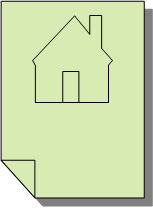
\includegraphics[width=0.25\textwidth]{Homepage-icon.png}
  \end{center}
  \caption{Homepage icon}
  \label{fig:homepageicon}
\end{figure}

\begin{table}[!ht]
  \begin{center}
    \caption{Configurations tested}
    \label{tab:configstested}
    \begin{tabular}{l|c} % <-- Alignments: 1st column left, 2nd middle and 3rd right, with vertical lines in between
      \textbf{Configuration} & \textbf{Description} \\
      \hline
      1 & Simple test with one server\\
      2 & Simple test with one server\\
    \end{tabular}
  \end{center}
\end{table}
\todo[inline, backgroundcolor=aqua]{Konfigurationer testade}

\section{Implementation …/Modeling/Simulation/…}
\todo[inline, backgroundcolor=aqua]{Implementering … / modellering / simulering / …}
\label{sec:implementationDetails}

\subsection{Some examples of coding}

Listing~\ref{lst:helloWorldInC} shows an example of a simple program written
in C code.

\begin{lstlisting}[language={C}, caption={Hello world in C code}, label=lst:helloWorldInC]
int main() {
printf("hello, world");
return 0;
}
\end{lstlisting}


In contrast, Listing~\ref{lst:programmes} is an example of code in Python to
get a list of all of the programs at KTH.

\lstset{extendedchars=true}
\begin{lstlisting}[language={Python}, caption={Using a python program to
    access the KTH API to get all of the programs at KTH}, label=lst:programmes]
KOPPSbaseUrl = 'https://www.kth.se'

def v1_get_programmes():
    global Verbose_Flag
    #
    # Use the KOPPS API to get the data
    # note that this returns XML
    url = "{0}/api/kopps/v1/programme".format(KOPPSbaseUrl)
    if Verbose_Flag:
        print("url: " + url)
    #
    r = requests.get(url)
    if Verbose_Flag:
        print("result of getting v1 programme: {}".format(r.text))
    #
    if r.status_code == requests.codes.ok:
        return r.text           # simply return the XML
    #
    return None
\end{lstlisting}


\cleardoublepage
\chapter{Results and Analysis}
\todo[inline, backgroundcolor=aqua]{svensk: Resultat och Analys}
\label{ch:resultsAndAnalysis}
\todo[inline]{
Sometimes this is split into two chapters.\\
  
Keep in mind: How you are going to evaluate what you have done? What are your metrics?\\
Analysis of your data and proposed solution\\
Does this meet the goals which you had when you started?
}

In this chapter, we present the results and discuss them.

\begin{swedishnotes}
I detta kapitel presenterar vi resultatet och diskutera dem.
\end{swedishnotes}
\todo[inline, backgroundcolor=aqua]{
Ibland delas detta upp i två kapitel.\\
Hur du ska utvärdera vad du har gjort? Vad är din statistik?\\
Analys av data och föreslagen lösning\\
Innebär detta att uppnå de mål som du hade när du började?
}

\section{Major results}
\todo[inline, backgroundcolor=aqua]{Huvudsakliga resultat}

Some statistics of the delay measurements are shown in Table~\ref{tab:delayMeasurements}.
The delay has been computed from the time the GET request is received until the response is sent.

\begin{swedishnotes}
Lite statistik av mätningarna fördröjnings visas i Tabell~\ref{tab:delayMeasurements}. Förseningen har beräknats från den tidpunkt då begäran GET tas emot fram till svaret skickas.
\end{swedishnotes}

\begin{table}[!ht]
  \begin{center}
    \caption{Delay measurement statistics}
    \label{tab:delayMeasurements}
    \begin{tabular}{l|S[table-format=4.2]|S[table-format=3.2]} % <-- Alignments: 1st column left, 2nd middle and 3rd right, with vertical lines in between
      \textbf{Configuration} & \textbf{Average delay (ns)} & \textbf{Median delay (ns)}\\
      \hline
      1 & 467.35 & 450.10\\
      2 & 1687.5 & 901.23\\
    \end{tabular}
  \end{center}
\end{table}
\todo[inline, backgroundcolor=aqua]{Fördröj mätstatistik}
\todo[inline, backgroundcolor=aqua]{Konfiguration | Genomsnittlig fördröjning (ns) | Median fördröjning (ns)}

Figure \ref{fig:processing_vs_payload_length} shows and example of the
performance as measured in the experiments.

\begin{figure}[!ht]
% GNUPLOT: LaTeX picture
\setlength{\unitlength}{0.240900pt}
\ifx\plotpoint\undefined\newsavebox{\plotpoint}\fi
\begin{picture}(1500,900)(0,0)
\sbox{\plotpoint}{\rule[-0.200pt]{0.400pt}{0.400pt}}%
\put(171.0,131.0){\rule[-0.200pt]{4.818pt}{0.400pt}}
\put(151,131){\makebox(0,0)[r]{ 1.5}}
\put(1419.0,131.0){\rule[-0.200pt]{4.818pt}{0.400pt}}
\put(171.0,212.0){\rule[-0.200pt]{4.818pt}{0.400pt}}
\put(151,212){\makebox(0,0)[r]{ 2}}
\put(1419.0,212.0){\rule[-0.200pt]{4.818pt}{0.400pt}}
\put(171.0,292.0){\rule[-0.200pt]{4.818pt}{0.400pt}}
\put(151,292){\makebox(0,0)[r]{ 2.5}}
\put(1419.0,292.0){\rule[-0.200pt]{4.818pt}{0.400pt}}
\put(171.0,373.0){\rule[-0.200pt]{4.818pt}{0.400pt}}
\put(151,373){\makebox(0,0)[r]{ 3}}
\put(1419.0,373.0){\rule[-0.200pt]{4.818pt}{0.400pt}}
\put(171.0,454.0){\rule[-0.200pt]{4.818pt}{0.400pt}}
\put(151,454){\makebox(0,0)[r]{ 3.5}}
\put(1419.0,454.0){\rule[-0.200pt]{4.818pt}{0.400pt}}
\put(171.0,534.0){\rule[-0.200pt]{4.818pt}{0.400pt}}
\put(151,534){\makebox(0,0)[r]{ 4}}
\put(1419.0,534.0){\rule[-0.200pt]{4.818pt}{0.400pt}}
\put(171.0,615.0){\rule[-0.200pt]{4.818pt}{0.400pt}}
\put(151,615){\makebox(0,0)[r]{ 4.5}}
\put(1419.0,615.0){\rule[-0.200pt]{4.818pt}{0.400pt}}
\put(171.0,695.0){\rule[-0.200pt]{4.818pt}{0.400pt}}
\put(151,695){\makebox(0,0)[r]{ 5}}
\put(1419.0,695.0){\rule[-0.200pt]{4.818pt}{0.400pt}}
\put(171.0,776.0){\rule[-0.200pt]{4.818pt}{0.400pt}}
\put(151,776){\makebox(0,0)[r]{ 5.5}}
\put(1419.0,776.0){\rule[-0.200pt]{4.818pt}{0.400pt}}
\put(171.0,131.0){\rule[-0.200pt]{0.400pt}{4.818pt}}
\put(171,90){\makebox(0,0){ 0}}
\put(171.0,756.0){\rule[-0.200pt]{0.400pt}{4.818pt}}
\put(298.0,131.0){\rule[-0.200pt]{0.400pt}{4.818pt}}
\put(298,90){\makebox(0,0){ 10}}
\put(298.0,756.0){\rule[-0.200pt]{0.400pt}{4.818pt}}
\put(425.0,131.0){\rule[-0.200pt]{0.400pt}{4.818pt}}
\put(425,90){\makebox(0,0){ 20}}
\put(425.0,756.0){\rule[-0.200pt]{0.400pt}{4.818pt}}
\put(551.0,131.0){\rule[-0.200pt]{0.400pt}{4.818pt}}
\put(551,90){\makebox(0,0){ 30}}
\put(551.0,756.0){\rule[-0.200pt]{0.400pt}{4.818pt}}
\put(678.0,131.0){\rule[-0.200pt]{0.400pt}{4.818pt}}
\put(678,90){\makebox(0,0){ 40}}
\put(678.0,756.0){\rule[-0.200pt]{0.400pt}{4.818pt}}
\put(805.0,131.0){\rule[-0.200pt]{0.400pt}{4.818pt}}
\put(805,90){\makebox(0,0){ 50}}
\put(805.0,756.0){\rule[-0.200pt]{0.400pt}{4.818pt}}
\put(932.0,131.0){\rule[-0.200pt]{0.400pt}{4.818pt}}
\put(932,90){\makebox(0,0){ 60}}
\put(932.0,756.0){\rule[-0.200pt]{0.400pt}{4.818pt}}
\put(1059.0,131.0){\rule[-0.200pt]{0.400pt}{4.818pt}}
\put(1059,90){\makebox(0,0){ 70}}
\put(1059.0,756.0){\rule[-0.200pt]{0.400pt}{4.818pt}}
\put(1185.0,131.0){\rule[-0.200pt]{0.400pt}{4.818pt}}
\put(1185,90){\makebox(0,0){ 80}}
\put(1185.0,756.0){\rule[-0.200pt]{0.400pt}{4.818pt}}
\put(1312.0,131.0){\rule[-0.200pt]{0.400pt}{4.818pt}}
\put(1312,90){\makebox(0,0){ 90}}
\put(1312.0,756.0){\rule[-0.200pt]{0.400pt}{4.818pt}}
\put(1439.0,131.0){\rule[-0.200pt]{0.400pt}{4.818pt}}
\put(1439,90){\makebox(0,0){ 100}}
\put(1439.0,756.0){\rule[-0.200pt]{0.400pt}{4.818pt}}
\put(171.0,131.0){\rule[-0.200pt]{0.400pt}{155.380pt}}
\put(171.0,131.0){\rule[-0.200pt]{305.461pt}{0.400pt}}
\put(1439.0,131.0){\rule[-0.200pt]{0.400pt}{155.380pt}}
\put(171.0,776.0){\rule[-0.200pt]{305.461pt}{0.400pt}}
\put(30,453){\rotatebox{-270}{\makebox(0,0){Processing time (ms)}}}
\put(805,29){\makebox(0,0){Payload size (bytes)}}
\put(868.0,131.0){\rule[-0.200pt]{0.400pt}{84.074pt}}
\put(995.0,131.0){\rule[-0.200pt]{0.400pt}{98.287pt}}
\put(1173.0,131.0){\rule[-0.200pt]{0.400pt}{118.041pt}}
\put(1325.0,131.0){\rule[-0.200pt]{0.400pt}{134.904pt}}
\put(1350.0,131.0){\rule[-0.200pt]{0.400pt}{137.795pt}}
\put(1439.0,131.0){\rule[-0.200pt]{0.400pt}{155.380pt}}
\end{picture}
\caption[A GNUplot figure]{Processing time vs. payload length}\vspace{0.5cm}
\label{fig:processing_vs_payload_length}
\end{figure}
		

Given these measurements, we can calculate our processing bit rate as the inverse of the time it takes to process an additional byte divided by 8 bits per byte:

\[
	bitrate = \frac{1}{\frac{time_{byte}}{8}} = 20.03 \quad kb/s
\] 

\section{Reliability Analysis}
\todo[inline, backgroundcolor=aqua]{Analys av reabilitet}
\begin{swedishnotes}
Reabilitet i metod och data 
\end{swedishnotes}

\section{Validity Analysis}
\todo[inline, backgroundcolor=aqua]{Analys av validitet}
\begin{swedishnotes}
Validitet i metod och data 
\end{swedishnotes}

\cleardoublepage
\chapter{Discussion}\todo[inline]{This can be a separate chapter or a section
  in the previous chapter.}
\todo[inline, backgroundcolor=aqua]{Diskussion}
\label{ch:discussion}
\begin{swedishnotes}
Förbättringsförslag?
\end{swedishnotes}

\cleardoublepage
\chapter{Conclusions and Future work}
\todo[inline, backgroundcolor=aqua]{Slutsats och framtida arbete}
\label{ch:conclusionsAndFutureWork}
Add text to introduce the subsections of this chapter.

\section{Conclusions}
\todo[inline]{Describe the conclusions (reflect on the whole introduction given in Chapter 1).}
\todo[inline, backgroundcolor=aqua]{Slutsatser}
\label{sec:conclusions}
  
Discuss the positive effects and the drawbacks.\\
Describe the evaluation of the results of the degree project.\\
Did you meet your goals?\\
What insights have you gained?\\
What suggestions can you give to others working in this area?\\
If you had it to do again, what would you have done differently?\\

\begin{swedishnotes}
Träffade du dina mål?
Vilka insikter har du fått?
Vilka förslag kan du ge till andra som arbetar inom detta område?
Om du hade att göra igen, vad skulle du ha gjort annorlunda?
\end{swedishnotes}

\section{Limitations}
\todo[inline]{What did you find that limited your
  efforts? What are the limitations of your results?}
\todo[inline, backgroundcolor=aqua]{Begränsande faktorer}
\label{sec:limitations}
\begin{swedishnotes}
Vad gjorde du som begränsade dina ansträngningar? Vilka är begränsningarna i dina resultat?
\end{swedishnotes}

\section{Future work}
\todo[inline]{Describe valid future work that you or someone else could or should do.\\
Consider: What you have left undone? What are the next obvious things to be done? What hints can you give to the next person who is going to follow up on your work?
}
\todo[inline, backgroundcolor=aqua]{Vad du har kvar ogjort?\\
Vad är nästa självklara saker som ska göras?\\
Vad tips kan du ge till nästa person som kommer att följa upp på ditt arbete?
}
\label{sec:futureWork}

Due to the breadth of the problem, only some of the initial goals have been
met. In these section we will focus on some of the remaining issues that
should be addressed in future work. ...

\subsection{What has been left undone?}
\label{what-has-been-left-undone}

The prototype does not address the third requirment, i.e., a yearly
unavailability of less than 3 minutes, this remains an open problem. ...

\subsubsection{Cost analysis}

The current prototype works, but the performance from a cost perspective makes
this an impractical solution. Future work must reduce the cost of this
solution, to do so a cost analysis needs to first be done. ...

\subsubsection{Security}

A future research effort is needed to address the security holes that results
from using a self-signed certificate. Page filling text mass. Page filling
text mass. ...


\subsection{Next obvious things to be done}

In particular, the author of this thesis wishes to point out xxxxxx remains as
a problem to be solved. Solving this problem is the next thing that should be
done. ...

\section{Reflections}
\todo[inline]{What are the relevant economic, social,
  environmental, and ethical aspects of your work?
}
\todo[inline, backgroundcolor=aqua]{Reflektioner}
\todo[inline, backgroundcolor=aqua]{Vilka är de relevanta ekonomiska, sociala, miljömässiga och etiska aspekter av ditt arbete?}
\label{sec:reflections}

One of the most important results is the reduction in the amount of
energy required to process each packet while at the same time reducing the
time required to process each packet.

The thesis contributes to the \gls{UN}\enspace\glspl{SDG} numbers 1 and 9 by
xxxx. 




\noindent\rule{\textwidth}{0.4mm}
\todo[inline]{In the references, let Zotero or other tool fill this
  in for you. I suggest an extended version of the IEEE  style, to include
  URLs, DOIs, ISBNs, etc., to make it easier for your reader to find
  them. This will make life easier for your opponents and examiner. \\

  IEEE Editorial Style Manual: \url{https://www.ieee.org/content/dam/ieee-org/ieee/web/org/conferences/style_references_manual.pdf}
}
\todo[inline, backgroundcolor=aqua]{Låt Zotero eller annat verktyg fylla i det här för dig. Jag föreslår en utökad version av IEEE stil - att inkludera webbadresser, DOI, ISBN etc. - för att göra det lättare för läsaren att hitta dem. Detta kommer att göra livet lättare för dina motståndare och examinator.}

\cleardoublepage
% Print the bibliography (and make it appear in the table of contents)
%\printbibliography[heading=bibintoc]
% The lines below are for BibTeX
\bibliographystyle{myIEEEtran}
\renewcommand{\bibname}{References}
\addcontentsline{toc}{chapter}{References}
\bibliography{references}




\cleardoublepage
\appendix
\renewcommand{\chaptermark}[1]{\markboth{Appendix \thechapter\relax:\thinspace\relax#1}{}}
\chapter{Something Extra}
\todo[inline, backgroundcolor=aqua]{svensk: Extra Material som Bilaga}

\label{pg:lastPageofMainmatter}

\clearpage
\section*{For DIVA}
\divainfo{pg:lastPageofPreface}{pg:lastPageofMainmatter}
\end{document}
